\documentclass{article}

\usepackage{graphicx}
\usepackage{graphpap}


\usepackage{fancyhdr}



%%%%%%%%%%%%%%%%%%%%%%%%%%%%%%%%%%%%%%%%5
%
%  Set Up Margins

%%%%%%%%%%%%%%%%%%%%%%%%%%%%%%%%%%%%%%%%%%%%%%%%%
% include file for:
%      Critical Page setup dimensions
%            DO NOT MODIFY
%       (for help see "Latex Line by Line" p 260)
%
\setlength\oddsidemargin{0in}
\setlength\evensidemargin{0in}

\usepackage[left=0.98in, right=0.98in, top=1.0in, bottom=1.0in]{geometry}

% %Top Margin and header
% \setlength\voffset{-0.94in}
% \setlength\topmargin{0.25in}
% \setlength\headheight{0.25in}
% %\setlength\headwidth{6.5in}
% \setlength\headsep{0.25in}
% %Body
% \setlength\textwidth{6.5in}
% \setlength\textheight{9.50in}
% %Footer
% %\setlength\footheight{0.5in}
% \setlength\footskip{0.3750in}
% Line spacing for 6 lines per inch
\linespread{0.894}  % 1.0 = single    1.6 = double
%
%          END of Critical Page Setup Dimensions
%%%%%%%%%%%%%%%%%%%%%%%%%%%%%%%%%%%%%%%%%%%%%%%%%%%

%%%%%%%%%%%%%%%%%%%%%%%%%%%%%%%%%%%%%%%%%%%%%%%%%%%
%
% Useful style and math macros
%


\newcommand\Dfrac[2]{\frac{\displaystyle #1}{\displaystyle #2}}
\newcommand\beq{\begin{equation}}
\newcommand\eeq{\end{equation}}

\newcommand\bmat{\begin{bmatrix}}
\newcommand\emat{\end{bmatrix}}

\newenvironment{solution}
{\vspace{0.125in} {\bf SOLUTION:} \\ }
{\vspace{0.25in}}



%%%%%%%%%%%%%%%%%%%%%%%%%%%%%%%%%%%%%%%%%%%%%%%%%
%
%         Page format Mods HERE
%
%Mod's to page size for this document
\addtolength\textwidth{0cm}
\addtolength\oddsidemargin{0cm}
\addtolength\headsep{0cm}
\addtolength\textheight{0cm}
%\linespread{0.894}   % 0.894 = 6 lines per inch, 1 = "single",  1.6 = "double"

%%%%%%%%%%%%%%%%%%%%%%%%%%%%% HEADER / FOOTER
\pagestyle{fancy}
%%%%%  Page header/footer fields for "NSF Style" proposal
%%%%%  \chead will be changed with each section
\lhead{\small\sc EE543}
\rhead{}
\chead{Problem Set 2}
\lfoot{Hannaford, U. of Washington}
\rfoot{\today}
\cfoot{\thepage}
%\renewcommand\headrulewidth{1pt}
%\renewcommand\footrulewidth{1pt}

\begin{document}

\setcounter{section}{1}
%%%%** Section 1
\section{Problem Set 2}

\subsection{} 
Draw or solve the common normals for each set of axes $A,B$ below

\subsubsection{}

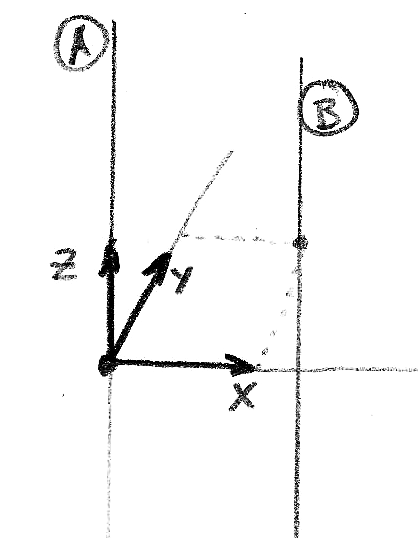
\includegraphics[width=1.50in]{hw2_W13_P1a.png}

A is equal to $Z$ axis.

$B = [2 \quad 2 \quad z]^T$

Unique?   \_\_\_ Yes  \_\_\_ No

\subsubsection{}

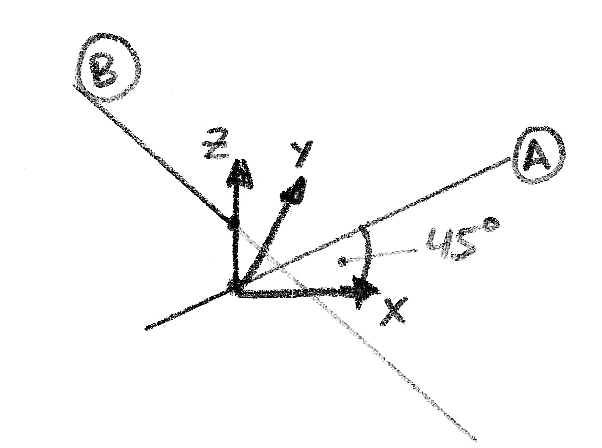
\includegraphics[width=2.50in]{hw2_W13_P1b.png}

A is in the $XY$ plane.

B is perpendicular to $Z$ axis. 

Unique?   \_\_\_ Yes  \_\_\_ No

\subsubsection{}

Make a drawing and find the Common Normal for:

A = $Y$ axis.

B = $[x \quad 3.0+0.8x \quad 5]^T$.

Unique?   \_\_\_ Yes  \_\_\_ No


\newpage
\subsection{}

Draw Common Normals and assign link frames for the following manipulator:

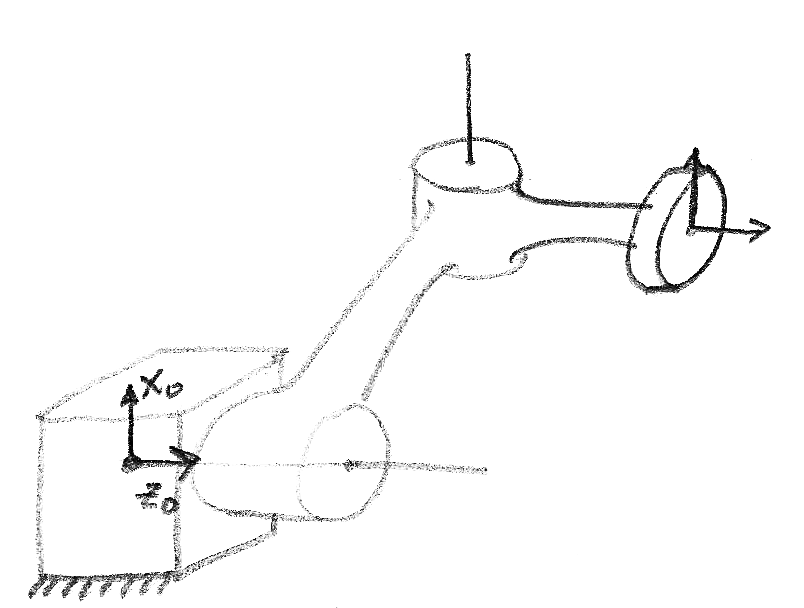
\includegraphics[width=4.0in]{hw2_W13_P2.png}

\subsection{}

Draw Common Normals and assign link frames for the following manipulator:

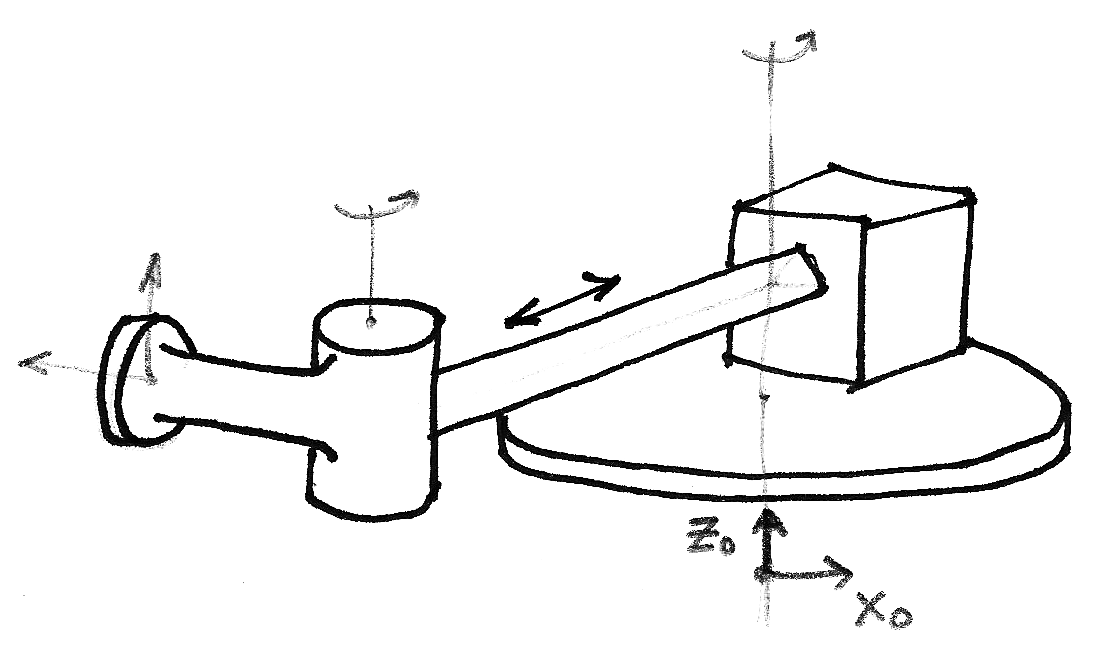
\includegraphics[width=4.0in]{hw2_W13_P3.png}


\end{document}

